\section{Strimzi}
\label{03:title}

This section describes the fundamental parts of the Strimzi project.
Moreover, it explains the whole architecture with all Operators (i.e., Topic, User, Cluster).
The description is based mainly on Strimzi documentation and blog posts\cite{strimziDoc, strimziBlogPosts}.

The information described in Sections~\ref{01:sec:title},~\ref{02:sec:title} was a precursor to a complete understanding of the Strimzi system.
Strimzi is an Apache Kafka orchestrator in the Kubernetes environment.
Therefore it is a collection of operators that simplify working with Kafka.
The Operator in Kubernetes is a component that is always in one of the following three states:
\begin{itemize}[itemsep=1mm, parsep=0pt]
    \item \textbf{Observe} \---\ gain the desired and current state,
    \item \textbf{Analysis} \---\ compares these two states and finds the differences,
    \item \textbf{Act} \---\ subsequently, if the given differences were found, it will do a reconciliation that will make the current and desired state identical
\end{itemize}

One can understand these Operators as a superset of the Deployment controller, which, like other controllers, followed the~\ref{01:alg:controllerAlg} algorithm.
The main difference is that the Operator oversees \emph{Custom Resources - CR}.
A Custom Resource is an extension of the Kubernetes API. These CRs define application objects in the Kubernetes environment.
Moreover, this is associated with the \emph{Custom Resource Definition}, which declares what values and types a given Custom Resource can acquire.
We can also imagine that Custom Resource Definition is a template comparable to classes in the Object-Oriented programming world, and Custom Resource is an instance of the class.
Strimzi defines a Custom Resource Definition for each Kafka component we described in section~\ref{02:sec:title} except for clients.
For example, for the KafkaBroker component, Strimzi has Kafka Custom Resource Definition.

\begin{figure}[!h]
    \hspace{0.01\textwidth}
    \subfigure[Example of Kafka Custom Resource Definition (Unnecessary parts omitted for brevity).]
        {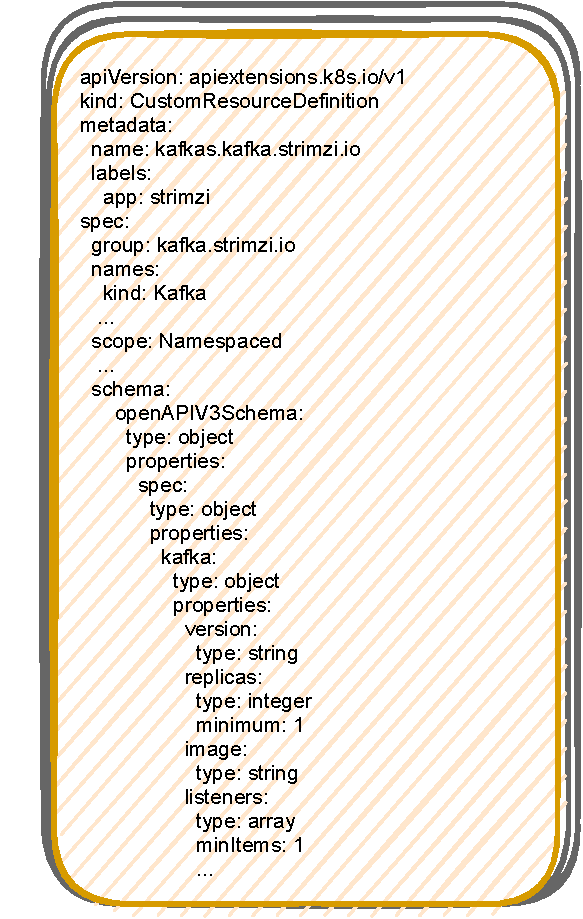
\includegraphics[scale=0.8]{obrazky-figures/02-preliminaries/03-strimzi/01-kafka-crd}}
    \label{03:fig:kafkacrds}
    \hspace{0.01\textwidth}
    \subfigure[Example of Kafka Custom Resource]
    {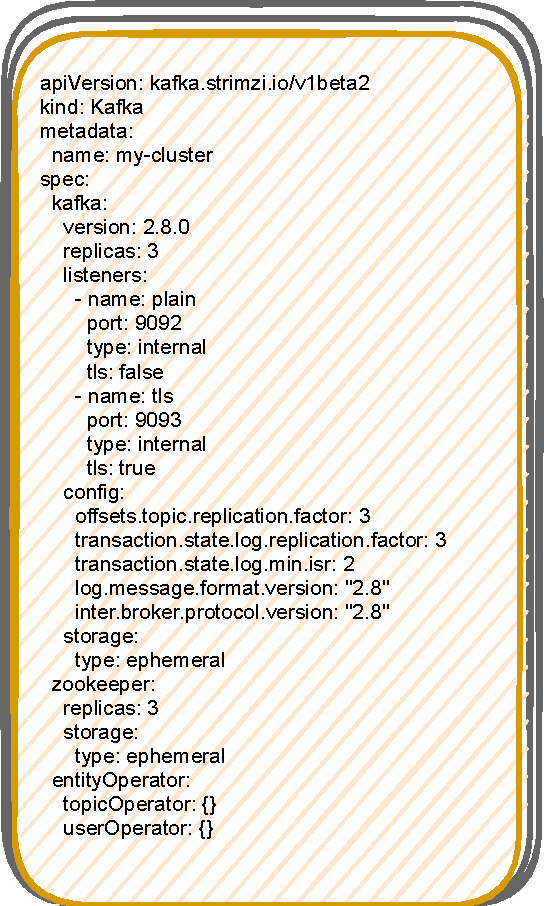
\includegraphics[scale=0.8]{obrazky-figures/02-preliminaries/03-strimzi/02-kafka-cr}}
    \label{03:fig:kafkacr}
    \hspace{0.01\textwidth}
    \caption{Kafka Custom Resource Definition and Kafka Custom Resource (Class and Instance)}
    \label{03:strimzi:fig:crds}
\end{figure}

Figure~\ref{03:strimzi:fig:crds} illustrates the mentioned Custom Resource and Custom Resource Definitions.
In Figure~\ref{03:strimzi:fig:crds} (left side), one can see Kafka Custom Resource Definition that shows several essential parts:
\begin{itemize}[itemsep=1mm, parsep=0pt]
    \item \textbf{labels.app.strimzi}  \---\ every Kafka Custom Resource in Kubernetes contains this label, and with that, it is easier to find these resources
    \item \textbf{spec.names.kind.Kafka} \---\ by this attribute, we specify how the Custom Resource type will be uniquely named.
    In this case, the label is Kafka.
    \item \textbf{spec.scope.Namespaced} \---\ type of environment scope.
    It distinguishes between Custom Resource, which works multi-namespace or single-namespace.
    Because Kafka Custom resource has value Namespaced (single-namespace), it can work in one namespace.
    On the other hand, we also know the Custom Resource can have the scope set to cluster (multi-namespace), which means they will observe all the namespaces that the Kubernetes cluster has.
    \item \textbf{spec.schema} \---\ this is the whole declaration of the Custom Resource Definition.
    In the child nodes, we can see what types the individual attributes must comply with and the restrictions on the given types.
    For example, the attribute \emph{replicas} has a restriction that it must be at least one and similarly for other attributes (it can not be zero).
\end{itemize}

On the other hand, we have Kafka Custom Resource (Figure~\ref{03:strimzi:fig:crds} - right side), which includes parts worth mentioning:
\begin{itemize}[itemsep=1mm, parsep=0pt]
    \item \textbf{apiVersion} \---\ This is the REST API offered by the Custom Resource Definition.
    The prefix must also match the value found in Kafka Custom Resource Definition in spec: group.
    \item \textbf{metadata.name} \---\ Custom Resource name,
    \item \textbf{spec.kafka.version} \---\ version of Kafka to be used,
    \item \textbf{spec.kafka.replicas} \---\ number of Kafka Pods to be deployed,
    \item \textbf{spec.kafka.listeners} \---\ types of listeners to be supported by a given Kafka instance.
    In this case, we see two types, one with plain communication listening on port 9092, and the second listener with encrypted communication using TLS technology and listening on port 9093.
    \item  \textbf{spec.kafka.config} \---\ these are additional configuration features that are added to Kafka (i.e., broker.id, log.dirs, zookeeper.connect, compression.type, cleanup.policy, delete.retention.ms),
    \item  \textbf{spec.kafka.storage}~\cite{strimziStorageBlogPost} \---\ the storage type.
    Kubernetes supports two storage types.
    In Figure~\ref{03:strimzi:fig:crds}, it is ephemeral storage.
    Ephemeral storage is usually a directory somewhere in the operating system on our Kubernetes node.
    It works the same as a temporary directory.
    There are also risks associated with this; if the Kubernetes node crashes, then the data stored in the ephemeral storage will be lost.
    The same thing will happen if we get a running Pod that will use ephemeral storage.
    In case of a restart, together with the new Pod, empty storage will be created, not containing the previous data.
    The second type of storage is Persistent, which eliminates these risks.
    \item \textbf{spec.zookeeper.replicas} \---\ number of Zookeeper Pods to be deployed,
    \item \textbf{spec.entityOperator} \---\ configuration for Entity Operator.
\end{itemize}

\subsection{Architecture}

Strimzi's architecture consists of two central units where the first unit is the Kafka architecture and the other components with which it communicates.
The second unit is the Operators architecture, consisting of a Cluster Operator, an Entity Operator, a Topic Operator, and a User Operator.
These Operators each have control loops, which control the already defined Custom Resources. (i.e, Kafka User, Kafka Topic, Kafka and Kafka Connect, Kafka Bridge, Kafka Mirror Maker, Kafka Mirror Maker 2, Kafka Rebalance)

The Kafka Architecture consists of several components, each performing specific tasks.
Zookeeper is one of the most significant dependencies for Kafka and limits it in several areas, scalability, metadata management and Deployment itself.
The answer to these problems came in a 2020 Kafka Improvement Proposal (KIP)\footnote{KIP-500 \---\ removal of Zookeeper with replacing him with self-managed metadata quorum \url{https://cwiki.apache.org/confluence/display/KAFKA/KIP-500}}.
As a result, Kafka 3.0 should run without Zookeeper.
Its responsibilities include, for example, leader election of partitions or storing the status of Kafka Brokers or Consumer offsets.
Clients in Figure~\ref{03:fig:strimziKafkaArchitecture} are classically Producer and Consumer as we know from the section~\ref{02:sec:title}, so their objective is clear.
On the other hand, HTTP clients communicate with the Kafka Bridge (a component provided by Strimzi) and thus connect the Kafka cluster and the clients themselves.
\begin{figure}[!ht]
    \centering
    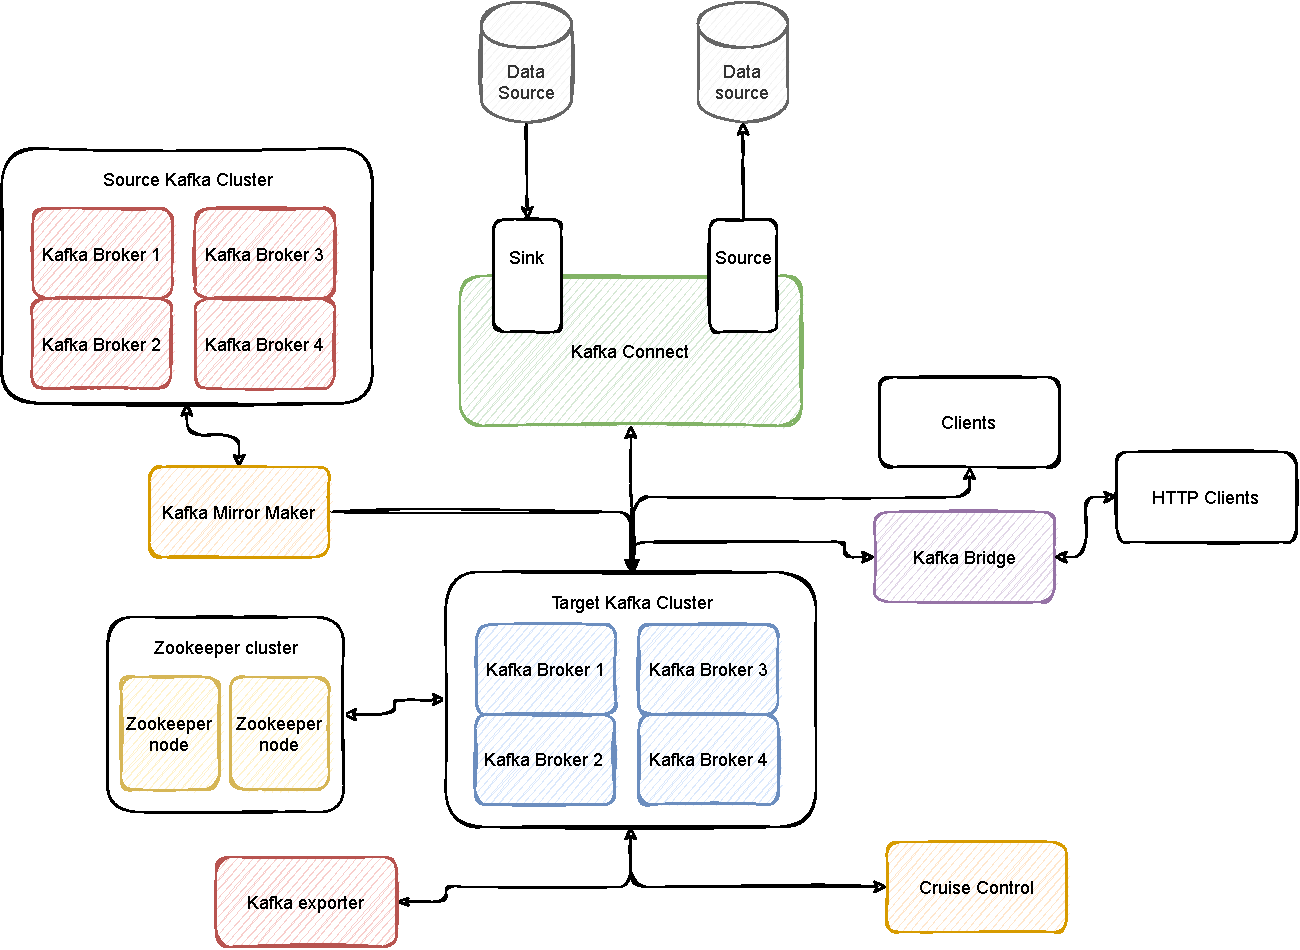
\includegraphics[scale=0.70]{obrazky-figures/02-preliminaries/03-strimzi/03-strimzi-kafka-architecture (1)}
    \caption{Strimzi Kafka architecture}
    \label{03:fig:strimziKafkaArchitecture}
\end{figure}
It communicates by default via the REST API, and the user can create, delete, and update Consumer, Producer, Topic and similar resources that Kafka Bridge offers.
So Kafka Bridge is nothing more than an HTTP proxy that integrates HTTP clients with a Kafka cluster.
Another part of the Kafka architecture is the Kafka Exporter, which is used to extract additional metrics and supply them to Prometheus\footnote{Prometheus \---\ open-soured metrics-based project. Moreover, it provides an alerting system with incredible features, in case of interest \url{https://prometheus.io/}}.
Then we have Kafka Connect and Kafka Mirror Maker, where we described the meaning of these components in Section~\ref{02:sec:title}.
The last essential component, especially for the overall balancing of the Kafka cluster, is Cruise Control.
This component collects data on CPU usage, partitions status, and many other metrics.
Cruise Control creates a workload model and analyses it when necessary to perform balancing and rearrange the load across the Kafka cluster.
Everything we have described is shown in Figure~\ref{03:fig:strimziKafkaArchitecture}.

The second part of the Strimzi architecture is the collection of Operators.
In the beginning, we described what such an Operator does (reconciliation/control loop).
Strimzi contains three Operators, where hierarchically, the highest is Cluster Operator.
This manages Kafka, Kafka Mirror Maker, Kafka Mirror Maker 2, Kafka Connect, Kafka Connector, Kafka Rebalance, and Kafka Bridge Custom Resources.
Furthermore, since Kafka Custom Resource encapsulates the Entity Operator (Topic and User Operator running within the same Pod but in different containers) and Zookeeper, the Operators mentioned above are also deployed with each Kafka Custom Resource deployment.
Figure~\ref{03:fig:strimziOperatorsArchitecture} illustrates whole Strimzi ecosystem, for which the Cluster Operator is responsible.

\begin{figure}[!ht]
    \centering
    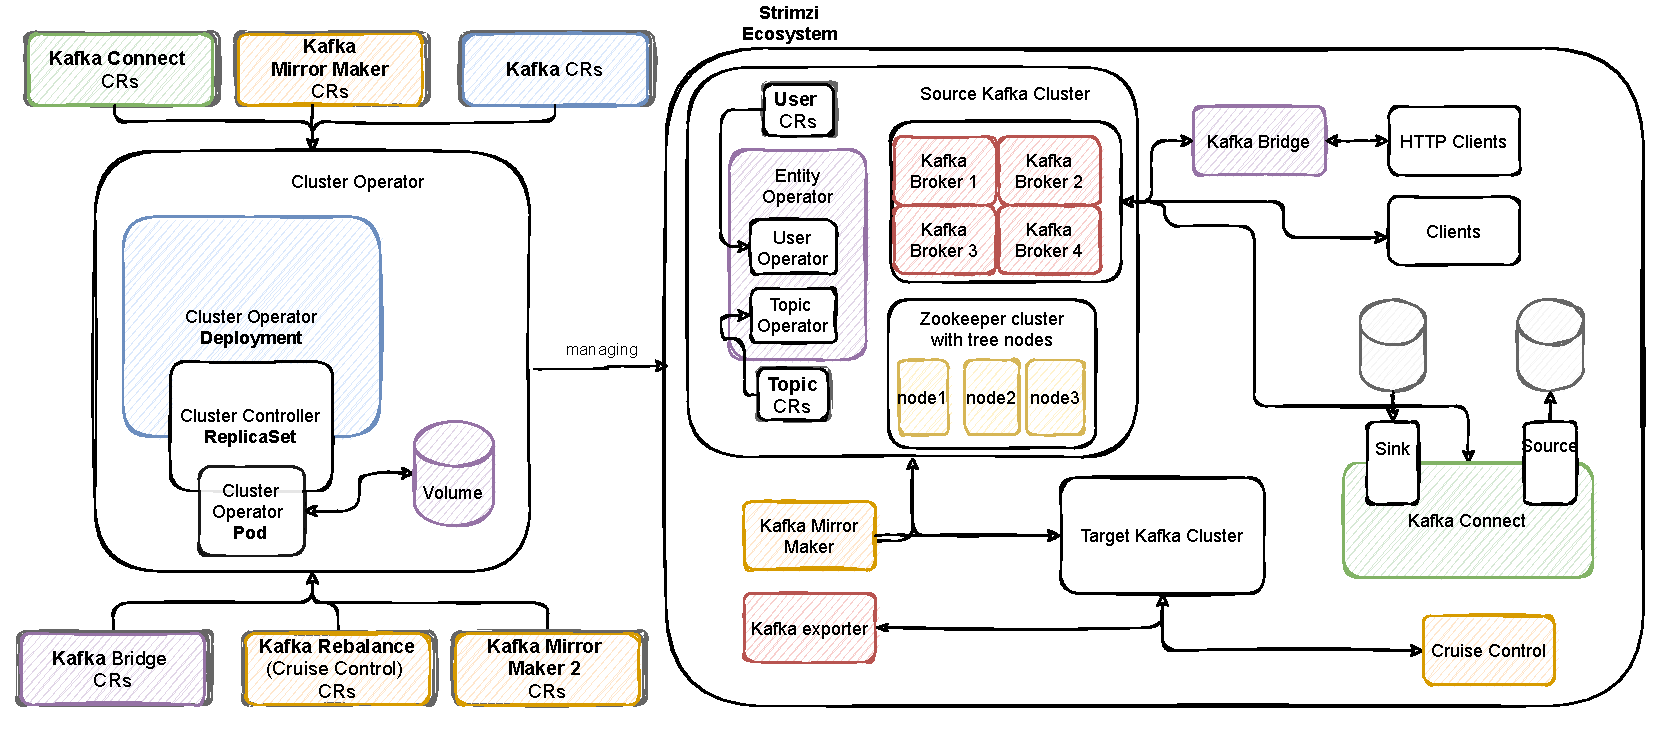
\includegraphics[scale=0.55]{obrazky-figures/02-preliminaries/03-strimzi/04-stirmziOperatorsArch}
    \caption{Strimzi Operators architecture with Strimzi ecosystem}
    \label{03:fig:strimziOperatorsArchitecture}
\end{figure}

The Topic Operator takes care of creating, deleting and updating individual Topics.
It is also necessary to mention that the Topic Operator ensures synchronisation between the Custom Resource Topic and the Topic located inside Kafka and keeps them in sync.
Strimzi documentation says - \emph{For instance, assume the scenario where the user changes different topic properties in Kubernetes
but simultaneously in Kafka itself. Also, imagine another scenario where one changes topic property simultaneously. The first action is considered allowed, and the solution for this is a 3-way diff (more about this method in section 2.19). In general, this method constructs these two differences' union and finds out where the intersection is not empty. The second one is treated as incompatible change. It must be deterministically selected by some winner policy implemented inside Topic Operator}.

The User Operator is responsible for the Kafka User Resource, which specifies authentication and authorisation for individual components.
It can be, for example, the Producer that can not change data in a Topic with a particular name or prefix.
In other words, we can define read and write rules for Topics.
In addition, we can create different types of Kafka Users, which support authentication such as TLS or SCRAM-SHA. Nevertheless, if we use SCRAM-SHA authentication, we must also configure one of the Kafka Broker listeners.
When one creates Kafka Custom Resource, then immediately the User Operator creates an associated Secret with the credentials.
These credentials are then submitted to the Consumer or Producer configuration.
Credentials ensure that the Producer or Consumer can connect to Kafka Broker and send or receive messages.
Several components can also be used in authorisation, such as ACLs (access control lists).
There is support for the Keycloak or Hydra authorisation server for more complex rules.
Another exciting feature is User quotas, ensuring that one client will never overload the entire Kafka Broker, and the total load will be limited.